\documentclass[reprint,aps,unsortedaddress,superscriptaddress,prd,floatfix,showpacs,linenumbers]{revtex4-2}
\usepackage[utf8]{inputenc}
\usepackage{float}
\usepackage{graphicx}
\usepackage{amsmath,amsthm,amssymb}
\usepackage{verbatim}
\usepackage{url}
\usepackage{subcaption}
\usepackage[separate-uncertainty=true]{siunitx}
\usepackage{physics}
\usepackage[]{hyperref}
\usepackage{cleveref}
\usepackage[obeyFinal]{todonotes}
\setuptodonotes{inline}
\graphicspath{{figures/}}
\DeclareSIUnit\barn{b}

\begin{document}
\title{Measurement of $(p+d)$ and $(p+p)$ cross section for
	$J/\Psi$ and $\Psi^\prime$ production at \SI{120}{\GeV}}
\affiliation{Department of Engineering and Physics, Abilene Christian
University, Abilene, Texas 79699, USA}
\affiliation{Institute of Physics, Academia Sinica, Taipei, 11529, Taiwan}
\affiliation{Physics Division, Argonne National Laboratory, Lemont,
Illinois 60439, USA}
\affiliation{Fermi National Accelerator Laboratory,
Batavia, Illinois 60510, USA}
\affiliation{Lawrence Berkeley National Laboratory, Berkeley, California,
94720, USA}
\affiliation{Physics Division, Los Alamos National Laboratory, Los Alamos,
New Mexico 97545, USA}
\affiliation{Institute of Particle and Nuclear Studies, KEK, High Energy
Accelerator Research Organization, Tsukuba, Ibaraki 305-0801, Japan}
\affiliation{Department of Physics and Astronomy, Mississippi State
University, Mississippi State, Mississippi 39762, USA }
\affiliation{Department of Physics, National Kaohsiung Normal University,
Kaohsiung City 80201, Taiwan}
\affiliation{RIKEN Nishina Center for Accelerator-Based Science, Wako,
Saitama 351-0198, Japan}
\affiliation{Department of Physics and Astronomy, Rutgers, The State
University of New Jersey, Piscataway, New Jersey 08854, USA}
\affiliation{Department of Physics, Tokyo Institute of Technology, Meguro-ku,
Tokyo 152-8550, Japan}
\affiliation{Department of Physics, University of Colorado, Boulder,
Colorado 80309, USA}
\affiliation{Department of Physics, University of Illinois at Urbana-Champaign, Urbana, Illinois 61801, USA}
\affiliation{Department of Physics, University of Maryland, College Park,
Maryland 20742, USA}
\affiliation{Randall Laboratory of Physics, University of Michigan, Ann Arbor,
Michigan 48109, USA}
\affiliation{Department of Physics, Yamagata University, Yamagata City,
Yamagata 990-8560, Japan}
\affiliation{Kellogg Radiation Laboratory, California Institute of Technology,
Pasadena, California 91125, USA}

\author{C. Leung}
\affiliation{Department of Physics, University of Illinois at Urbana-Champaign,
Urbana, Illinois 61801, USA}

\author{J. Dove}
\affiliation{Department of Physics, University of Illinois at Urbana-Champaign,
Urbana, Illinois 61801, USA}

\author{B. Kerns}
\affiliation{Department of Physics, University of Illinois at Urbana-Champaign,
Urbana, Illinois 61801, USA}

\author{R. E. McClellan}
\affiliation{Department of Physics, University of Illinois at Urbana-Champaign,
Urbana, Illinois 61801, USA}

\author{S. Miyasaka}
\affiliation{Department of Physics, Tokyo Institute of Technology, Meguro-ku,
Tokyo 152-8550, Japan}

\author{D. H. Morton}
\affiliation{Randall Laboratory of Physics, University of Michigan, Ann Arbor,
Michigan 48109, USA}

\author{K. Nagai}
\affiliation{Department of Physics, Tokyo Institute of Technology, Meguro-ku,
Tokyo 152-8550, Japan}
\affiliation{Institute of Physics, Academia Sinica, Taipei, 11529, Taiwan}

\author{S. Prasad}
\affiliation{Department of Physics, University of Illinois at Urbana-Champaign,
Urbana, Illinois 61801, USA}

\author{F. Sanftl}
\affiliation{Department of Physics, Tokyo Institute of Technology, Meguro-ku,
Tokyo 152-8550, Japan}

\author{M. B. C. Scott}
\affiliation{Randall Laboratory of Physics, University of Michigan, Ann Arbor,
Michigan 48109, USA}

\author{A. S. Tadepalli}
\affiliation{Department of Physics and Astronomy, Rutgers, The State
University of New Jersey, Piscataway, New Jersey 08854, USA}

\author{C. A. Aidala}
\affiliation{Randall Laboratory of Physics, University of Michigan, Ann Arbor,
Michigan 48109, USA}
\affiliation{Physics Division, Los Alamos National Laboratory, Los Alamos,
New Mexico 97545, USA}

\author{J.  Arrington}
\affiliation{Physics Division, Argonne National Laboratory, Lemont,
Illinois 60439, USA}
\affiliation{Lawrence Berkeley National Laboratory, Berkeley, California,
94720, USA}

\author{C. Ayuso}
\affiliation{Randall Laboratory of Physics, University of Michigan, Ann Arbor,
Michigan 48109, USA}

\author{C. L. Barker}
\affiliation{Department of Engineering and Physics, Abilene Christian
University, Abilene, Texas 79699, USA}

\author{C. N. Brown}
\affiliation{Fermi National Accelerator Laboratory,
Batavia, Illinois 60510, USA}

\author{T. H. Chang}
\affiliation{Institute of Physics, Academia Sinica, Taipei, 11529, Taiwan}

\author{W. C. Chang}
\affiliation{Institute of Physics, Academia Sinica, Taipei, 11529, Taiwan}

\author{A. Chen}
\affiliation{Department of Physics, University of Illinois at Urbana-Champaign,
Urbana, Illinois 61801, USA}
\affiliation{Institute of Physics, Academia Sinica, Taipei, 11529, Taiwan}
\affiliation{Randall Laboratory of Physics, University of Michigan, Ann Arbor,
Michigan 48109, USA}

\author{D. C. Christian}
\affiliation{Fermi National Accelerator Laboratory,
Batavia, Illinois 60510, USA}

\author{B. P. Dannowitz}
\affiliation{Department of Physics, University of Illinois at Urbana-Champaign,
Urbana, Illinois 61801, USA}

\author{M. Daugherity}
\affiliation{Department of Engineering and Physics, Abilene Christian
University, Abilene, Texas 79699, USA}

\author{M. Diefenthaler}
\affiliation{Department of Physics, University of Illinois at Urbana-Champaign,
Urbana, Illinois 61801, USA}

\author{L. El Fassi}
\affiliation{Department of Physics and Astronomy, Mississippi State
University, Mississippi State, Mississippi 39762, USA }
\affiliation{Department of Physics and Astronomy, Rutgers, The State
University of New Jersey, Piscataway, New Jersey 08854, USA}

\author{D. F. Geesaman}
\affiliation{Physics Division, Argonne National Laboratory, Lemont,
Illinois 60439, USA}

\author{R. Gilman}
\affiliation{Department of Physics and Astronomy, Rutgers, The State
University of New Jersey, Piscataway, New Jersey 08854, USA}

\author{Y. Goto}
\affiliation{RIKEN Nishina Center for Accelerator-Based Science, Wako,
Saitama 351-0198, Japan}

\author{L. Guo}
\affiliation{Physics Division, Los Alamos National Laboratory, Los Alamos,
New Mexico 97545, USA}

\author{R. Guo}
\affiliation{Department of Physics, National Kaohsiung Normal University,
Kaohsiung City 80201, Taiwan}

\author{T. J. Hague}
\affiliation{Department of Engineering and Physics, Abilene Christian
University, Abilene, Texas 79699, USA}

\author{R. J. Holt}
\affiliation{Physics Division, Argonne National Laboratory, Lemont,
Illinois 60439, USA}
\affiliation{Kellogg Radiation Laboratory, California Institute of Technology,
Pasadena, California 91125, USA}

\author{D. Isenhower}
\affiliation{Department of Engineering and Physics, Abilene Christian
University, Abilene, Texas 79699, USA}

\author{E. R. Kinney}
\affiliation{Department of Physics, University of Colorado, Boulder,
Colorado 80309, USA}

\author{N. Kitts}
\affiliation{Department of Engineering and Physics, Abilene Christian
University, Abilene, Texas 79699, USA}

\author{A. Klein}
\affiliation{Physics Division, Los Alamos National Laboratory, Los Alamos,
New Mexico 97545, USA}

\author{D. W. Kleinjan}
\affiliation{Physics Division, Los Alamos National Laboratory, Los Alamos,
New Mexico 97545, USA}

\author{Y. Kudo}
\affiliation{Department of Physics, Yamagata University, Yamagata City,
Yamagata 990-8560, Japan}

\author{P.-J. Lin}
\affiliation{Department of Physics, University of Colorado, Boulder,
Colorado 80309, USA}

\author{K. Liu}
\affiliation{Physics Division, Los Alamos National Laboratory, Los Alamos,
New Mexico 97545, USA}

\author{M. X. Liu}
\affiliation{Physics Division, Los Alamos National Laboratory, Los Alamos,
New Mexico 97545, USA}

\author{W. Lorenzon}
\affiliation{Randall Laboratory of Physics, University of Michigan, Ann Arbor,
Michigan 48109, USA}

\author{N. C. R. Makins}
\affiliation{Department of Physics, University of Illinois at Urbana-Champaign,
Urbana, Illinois 61801, USA}

\author{ M. Mesquita de Medeiros}
\affiliation{Physics Division, Argonne National Laboratory, Lemont,
Illinois 60439, USA}

\author{P. L. McGaughey}
\affiliation{Physics Division, Los Alamos National Laboratory, Los Alamos,
New Mexico 97545, USA}

\author{Y. Miyachi}
\affiliation{Department of Physics, Yamagata University, Yamagata City,
Yamagata 990-8560, Japan}

\author{I. Mooney}
\affiliation{Randall Laboratory of Physics, University of Michigan, Ann Arbor,
Michigan 48109, USA}

\author{K. Nakahara}
\affiliation{Department of Physics, University of Maryland, College Park,
Maryland 20742, USA}

\author{K. Nakano}
\affiliation{Department of Physics, Tokyo Institute of Technology, Meguro-ku,
Tokyo 152-8550, Japan}
\affiliation{RIKEN Nishina Center for Accelerator-Based Science, Wako,
Saitama 351-0198, Japan}

\author{S. Nara}
\affiliation{Department of Physics, Yamagata University, Yamagata City,
Yamagata 990-8560, Japan}

\author{J. C. Peng}
\affiliation{Department of Physics, University of Illinois at Urbana-Champaign,
Urbana, Illinois 61801, USA}

\author{A. J. Puckett}
\affiliation{Physics Division, Los Alamos National Laboratory, Los Alamos,
New Mexico 97545, USA}

\author{B. J. Ramson}
\affiliation{Randall Laboratory of Physics, University of Michigan, Ann Arbor,
Michigan 48109, USA}
\affiliation{Fermi National Accelerator Laboratory,
Batavia, Illinois 60510, USA}

\author{P. E. Reimer}
\affiliation{Physics Division, Argonne National Laboratory, Lemont,
Illinois 60439, USA}

\author{J. G. Rubin}
\affiliation{Randall Laboratory of Physics, University of Michigan, Ann Arbor,
Michigan 48109, USA}
\affiliation{Physics Division, Argonne National Laboratory, Lemont,
Illinois 60439, USA}

\author{S. Sawada}
\affiliation{Institute of Particle and Nuclear Studies, KEK, High Energy
Accelerator Research Organization, Tsukuba, Ibaraki 305-0801, Japan}

\author{T. Sawada}
\affiliation{Randall Laboratory of Physics, University of Michigan, Ann Arbor,
Michigan 48109, USA}

\author{T.-A. Shibata}
\affiliation{Department of Physics, Tokyo Institute of Technology, Meguro-ku,
Tokyo 152-8550, Japan}
\affiliation{RIKEN Nishina Center for Accelerator-Based Science, Wako,
Saitama 351-0198, Japan}

\author{S. H. Shiu}
\affiliation{Institute of Physics, Academia Sinica, Taipei, 11529, Taiwan}

\author{D. Su}
\affiliation{Institute of Physics, Academia Sinica, Taipei, 11529, Taiwan}

\author{M. Teo}
\affiliation{Department of Physics, University of Illinois at Urbana-Champaign,
Urbana, Illinois 61801, USA}

\author{B. G Tice}
\affiliation{Physics Division, Argonne National Laboratory, Lemont,
Illinois 60439, USA}

\author{R. S. Towell}
\affiliation{Department of Engineering and Physics, Abilene Christian
University, Abilene, Texas 79699, USA}

\author{S. Uemura}
\affiliation{Department of Engineering and Physics, Abilene Christian
University, Abilene, Texas 79699, USA}

\author{S. Watson}
\affiliation{Department of Engineering and Physics, Abilene Christian
University, Abilene, Texas 79699, USA}

\author{S. G. Wang}
\affiliation{Institute of Physics, Academia Sinica, Taipei, 11529, Taiwan}
\affiliation{Department of Physics, National Kaohsiung Normal University,
Kaohsiung City 80201, Taiwan}

\author{A. B. Wickes}
\affiliation{Physics Division, Los Alamos National Laboratory, Los Alamos,
New Mexico 97545, USA}

\author{J. Wu}
\affiliation{Fermi National Accelerator Laboratory, Batavia, Illinois 60510, USA}

\author{Z. Xi}
\affiliation{Department of Engineering and Physics, Abilene Christian
University, Abilene, Texas 79699, USA}

\author{Z. Ye}
\affiliation{Physics Division, Argonne National Laboratory, Lemont,
Illinois 60439, USA}

\collaboration{FNAL E906/SeaQuest Collaboration}
\noaffiliation

\date{\today}
\begin{abstract}
	High-mass dimuon production in $p+p$ and $p+d$ interaction has been measured
	in the SeaQuest experiment with \SI{120}{\GeV} proton beam at Fermilab.
	We report the $(p+d) / (p+p)$ cross section
	ratios for $J/\Psi$ and $\psi^\prime$ production covering the forward
	rapidity region of $0.3 < x_F <0.8$. Unlike the recently reported
	$(p+d) / (p+p)$ Drell-Yan cross section ratios from SeaQuest, which are
	sensitive to the
	$\bar{d} / \bar{u}$ antiquark distributions in the proton, the corresponding
	cross section ratios for charmonium production are primarily
	sensitive to the gluon
	distributions in the proton and neutron. We compare the measured
	charmonium production cross section ratios with that of the
	Drell-Yan process. We also compare the measured cross section ratios with
	theoretical calculations.

	\todo[inlinewidth=12cm]{Should the focus be on the cross section or the ratio?}
\end{abstract}

\pacs{14.20.Dh,14.65.Bt,13.60.Hb}

\maketitle
\section{Introduction}
The SeaQuest experiment at Fermilab was designed to measure high-mass dimuons
produced in the interaction of \SI{120}{\GeV} proton beam with various targets
including liquid hydrogen and deuterium and solid nuclear targets. Dimuons
originating from the Drell-Yan process~\cite{drell1970} as well as from the decay of quarkonium
states ($J/\Psi$ and $\Psi^\prime$) have been collected simultaneously.
Results of the $(p+d) / (p+p)$ Drell-Yan cross section ratios, which are sensitive
to the flavor asymmetry of $\bar{d}/ \bar{u}$ in the proton, have been reported
recently~\cite{dove2021,dove2023}. In this paper, we report the
$p+p$ and $p+p$ cross section for the $J/\Psi$ and $\Psi^\prime$ charmonium production.

\todo{explain the interest of studying the charmomnium}
Unlike the Drell-Yan process which primarily involves the annihilation
of quark and antiquark pair via electromagnetic interaction, charmonium
production proceeds via strong interaction containing contributions from
both the quark-antiquark annihilation and the gluon-gluon
fusion processes. The simultaneous measurement of these two very different
processes, Drell-Yan and charmonium production, provides complimentary
information on the partonic structures of the nucleon.

From the consideration of charge symmetry (CS), which corresponds to an
invariance under a rotation of $180^\circ$ along the second axis of the
isospin space, the gluon distribution in the proton should be identical
to that of the neutron. This reflects the iso-scalar nature of the gluon.
Evidence for a small violation of charge symmetry has been
reported in some interactions
involving hadrons, such as the $d d \to {\pi^0}~^4\mbox{He}$
reaction~\cite{opper2003}
and the $n p \to \pi^0 d$ reaction~\cite{stephenson2003}.
Charge symmetry is also predicted to be violated at the
partonic level, although there exists no experimental evidence
so far for such violations~\cite{londergan2010}. A sensitive measurement of the
gluon contents in proton and deuteron could provide a test of CS at
the partonic level~\cite{piller1996,zhu2008}.

While proton-induced charmonium production is expected to be dominated
by the gluon-gluon fusion process~\cite{vogt1999}, some contributions from the
quark-antiquark annihilation process is also anticipated. The relative
importance of these two
processes is expected to depend on the total energy of the colliding hadrons
as well as the Feynman-$x$ ($x_F$) of the
charmonium~\cite{peng1995}. The quark-antiquark annihilation is sensitive to the
$\bar d / \bar u$ flavor asymmetry in the proton, while the
gluon-gluon fusion is expected to be similar for the reaction
on hydrogen and deuterium targets. Therefore, the $x_F$ dependence
of the $(p+d) / (p+p)$ cross section ratio for $J/\Psi$ production could reveal
the relative importance of these two processes.

The NA51 Collaboration reported a measurement of the $(p+d)$ and $ (p+p)$ cross
section for charmonium production at 450 GeV at a single value of
rapidity~\cite{abreu1998}. The present measurement covers the kinematic range
of $0.3 < x_F < 0.8$. The 120 GeV beam energy
in the SeaQuest experiment is expected to probe
the parton distribution at larger values of $x$, the fractional momentum
carried by the partons, than probed by the NA51 experiment at 450 GeV.

\todo{explain the scope of the paper}
The organization of this paper is as follows. Following this introduction, the
SeaQuest experiments will be described in \cref{sec:SeaQuest}. \Cref{sec:analysis}
will present the procedure for data analysis and Monte-Carlo simulation. Results
of the $x_F$ and $P_T$ dependencies of the $p+p$ and $p+d$ cross sections will
be presented in \cref{sec:cross_section}. The $(p+d)/(p+p)$ charmonium cross section
ratios will be compared with the Drell-Yan ratios in \cref{sec:CSR}, followed by a
conclusion.

\section{The SeaQuest Experiment}
\label{sec:SeaQuest}
\todo{brief discussion of the spectrometer}
The SeaQuest experiment was performed using a \SI{120}{\GeV} proton beam from the
Fermilab Main Injector. The SeaQuest dimuon spectrometer was designed for
detecting high-mass dimuon pairs produced in the interaction of proton
with various targets. Details of the SeaQuest spectrometer can be found
elsewhere~\cite{aidala2019}. A primary proton beam with up to $6 \times 10^{12}$
protons in a 4-second long spill every minute was incident upon one
of three identical 50.8-cm long cylindrical stainless steel
target flasks containing either liquid hydrogen, liquid deuterium,
or vacuum. The targets alternated between liquid hydrogen, liquid deuterium,
and the empty flask targets. A Beam Intensity Monitor (BIM) Cherenkov counter
was placed in the beam to record the instantaneous proton intensity for
each 1-ns long RF bucket at \SI{53}{\MHz} repetition rate. The BIM is essential
for measuring the integrated beam luminosity, and to inhibit triggers
occurring within RF buckets containing large number of protons
exceeding a preset threshold. This significantly reduces the data-acquisition
deadtime by rejecting at the trigger level those events which are potentially
too noisy to be reliably reconstructed.

The spectrometer consists of four detector stations containing
hodoscopes and tracking chambers.
Central to the spectrometer are two large dipole magnets.
The first magnet (FMag) downstream of the target is a solid iron 10
T-m focusing magnet which
also serves as a beam-dump and a hadron absorber. The second
magnet (KMag) placed between the first and second detector stations
provided a \SI{0.41}{\GeV/c} transverse momentum kick
for measuring the charge and momentum of the muons. Dimuon events
were triggered based on the requirement of a triple hodoscope
coincidence with a pattern consistent with a muon pair originating
from the target. Various diagnostic triggers were also implemented
for studying the spectrometer performance.

\section{Data Analysis}
\label{sec:analysis}
Tracks reconstructed in the drift chambers were extrapolated
to the target region using the momentum determined by
the KMag analyzing magnet. Only dimuon events consistent with originating
from the target, rather than from the beam dump, were selected with various
analysis cuts. For events surviving these analysis cuts, the target
position was then used to
refine the parameters of each muon pair. The resulting
RMS mass resolution for $J/\Psi$ is $\sim\SI{200}{\MeV}$.
This resolution is dominated by the finite target length and the
multiple scattering of muons in the iron magnet.

\todo{explain mass fit, refer to long paper}
\begin{figure}
	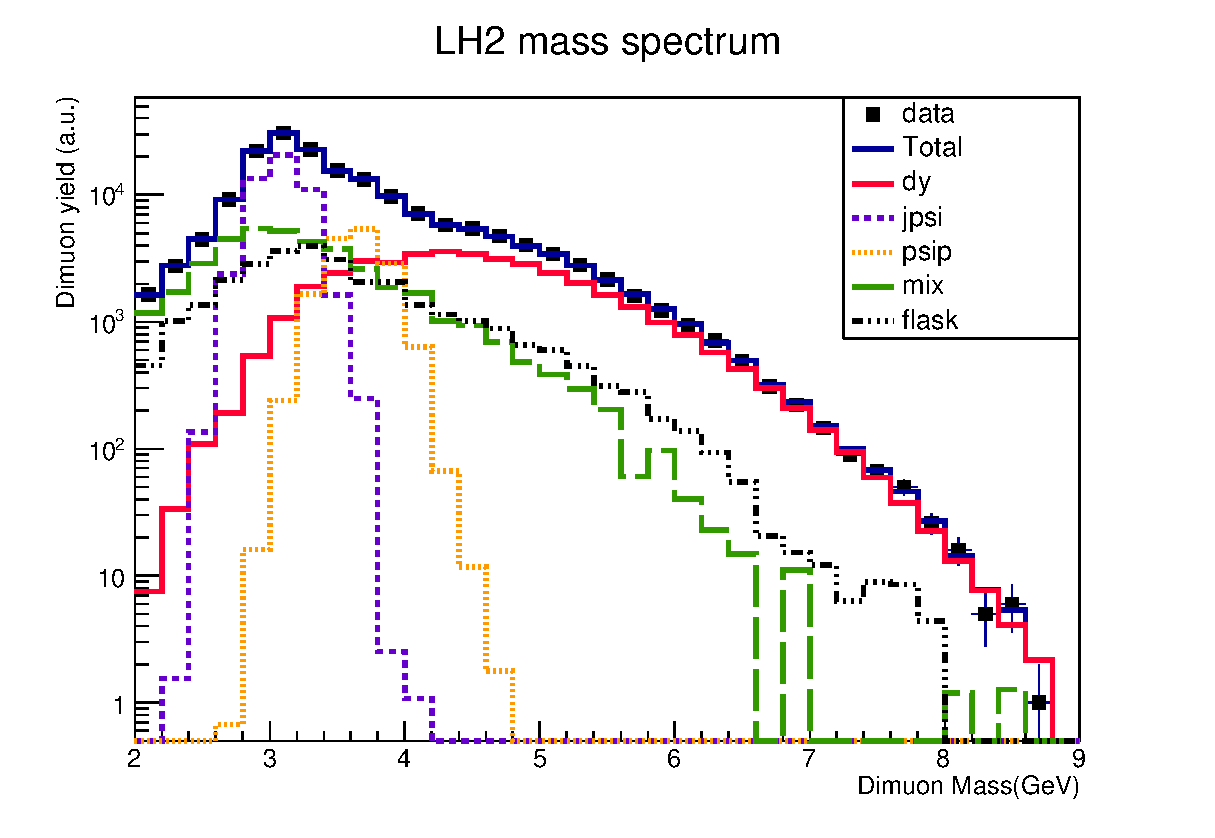
\includegraphics[width=\linewidth]{massFit/LH2_massfit}
	\todo{revisit style of massfit, might use figure in long paper}
	\caption{Dimuon mass distribution for data collected on liquid hydrogen target
		after all analysis cuts.}
	\label{fig:massfit_LH2}
\end{figure}
\Cref{fig:massfit_LH2} shows the dimuon mass spectrum for the data collected with the
liquid hydrogen target. In order to extract the yields of $J/\Psi$ and
$\Psi^\prime$, we performed a fit to the dimuon mass distribution taking
into account several contributions. First, the mass spectrum from the
data collected with empty target flask, properly normalized by the
integrated beam intensity, is shown as the dotted curve. Second, the
dimuon mass distributions for $J/\Psi$ and $\Psi^\prime$ are shown as
the solid curves. A detailed Monte-Carlo (M-C) simulation based on Geant was
performed to obtain the expected line shapes of the $J/\Psi$ and $\Psi^\prime$
resonances. The M-C simulation first generated the ``clean" dimuon events,
which were then embedded by the additional hits in the detectors according to
the data collected with the ``random" trigger. These embedded
so-called ``messy" M-C events were then analyzed by applying reconstruction
and target selection cuts identical to those applied to the real data. This
procedure ensures that the spectrometer responses to the background hits,
reflected in the "random" trigger data, are properly taken into account.
Third, the dimuons orginating from the Drell-Yan process are simulated
by the M-C, as shown in the dashed curve in \cref{fig:massfit_LH2}. These M-C
Drell-Yan events were generated using next-to-leading order
calculations and the CT14 parton distributions,
which reproduce the $\bar{d}/ \bar{u}$ asymmetry in the $x < 0.3$ region.
The same embedding procedure was also applied to the Drell-Yan M-C data.

\begin{figure}
	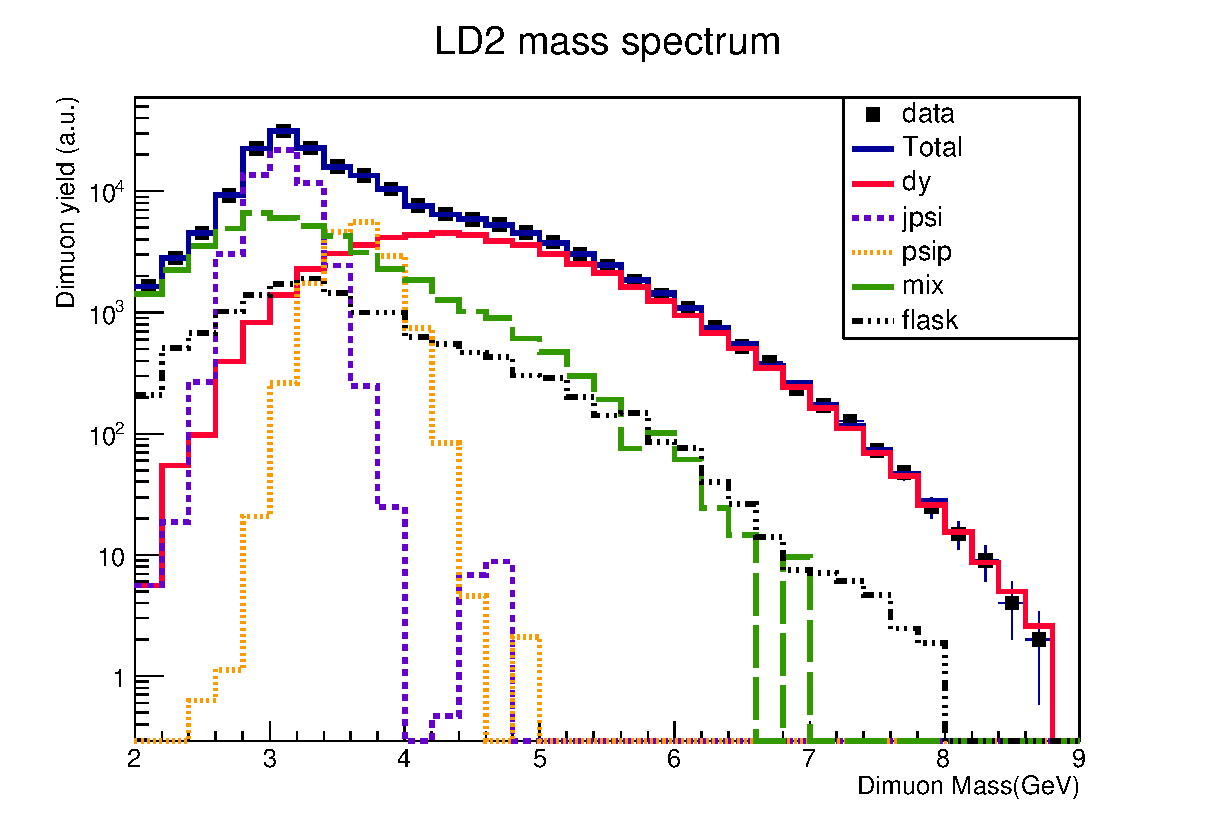
\includegraphics[width=\linewidth]{massFit/LD2_massfit}
	\todo{revisit style of massfit, might use figure in long paper}
	\caption{Same as \cref{fig:massfit_LH2}, but for data collected on the liquid
		deuterium target.}
	\label{fig:massfit_LD2}
\end{figure}

In addition to the above contributions to the dimuon events, an important
contribution is the accidental dimuon background caused by two charged
muons generated in two independent interactions from protons in the same
RF bucket with the target or other material. An extensive
study has been performed to determine the mass distribution of this background,
and we found that this background could be simulated by using
the data collected with the special ``single-muon" trigger. An analysis
of data formed by a random
comination of these single-muon tracks, weighted by the proper beam intensity
profile consistent with that for the dimuon events, is shown as the dot-dashed
curve in \cref{fig:massfit_LH2}. A fit to the dimuon data, allowing the normalizations of
the various components except the empty flask data to vary, is shown in \cref{fig:massfit_LH2}
as the solid curve. The data are well described by the combination of various
components. The adequacy of this approach is further supported by the excellent
agreement for the extracted Drell-Yan $(p+d) / (p+p)$ cross section ratio
between this method~\cite{dove2023} and an independent intensity-extrapolation
method adopted in Ref.~\cite{dove2021}.

\Cref{fig:massfit_LD2} shows the dimuon mass distribution for events passing all analysis
cuts for the data collected on the liquid deuterium target. The various curves
in \cref{fig:massfit_LD2} correspond to the different components analogous to those in \cref{fig:massfit_LH2}.
The good agreement between the data and the fit indicates the suitability of
this approach to extract the $J/\Psi$ and the $\Psi^\prime$ yields.

We recall the following definitions of the kinematic variable:
\begin{equation}
	x_F = \frac{P_L}{P_{max}}=\frac{2P_L}{\sqrt{s}\left(1-M^2/s\right)},
\end{equation}
where $P_L$ is the longitudinal momentum of the $J/\psi$ and $P_{max}$ is
the maximum momentum for the $J/\psi$ in the hadron-hadron center-of-mass
frame. $M$ and $\sqrt{s}$ are the $J/\psi$ mass and the hadron-hadron total energy,
respectively. From the $J/\psi$ four momentum $Q$, the variable $x_1$ and $x_2$
are obtained:
\begin{equation}
	x_1=\frac{P_2\cdot Q}{P_2 \cdot \left(P_1 + P_2\right)} \textrm{ and } x_2=\frac{P_1\cdot Q}{P_1 \cdot \left(P_1 + P_2\right)}
\end{equation}
where $P_1$ and $P_2$ are the four momenta of the projectile and target hadron,
respectively.

\section{\texorpdfstring{$J/\psi$}{J/psi} and \texorpdfstring{$\psi'$}{psi'} Cross Section}
\label{sec:cross_section}
\todo{describe the cross section calculation}
In order to obtain the $J/\Psi$ and $\psi'$ $d\sigma/dx_F$ differential cross sections,
the data were split into five bins of $x_F$ and the dimuon mass distributions
were fitted for each $x_F$ bin to extract the $J/\Psi$ and $\psi'$ yield.
The quarkonium production cross section is obtained from the yields ($Y$) as follows
\begin{equation}
	d\sigma = \frac{Y}{Acc \cdot Eff \cdot Lum},
	\label{eq:eq2}
\end{equation}
where $Acc$ is the spectrometer acceptance, $Eff$ the efficiency for
analysis cuts, and $Lum$ the effective luminosity including the
data-acquisition deadtime.
\todo{describe the extracted cross section and how it compared with predictions}
\begin{figure*}[h]
	\begin{subfigure}{0.45\linewidth}
		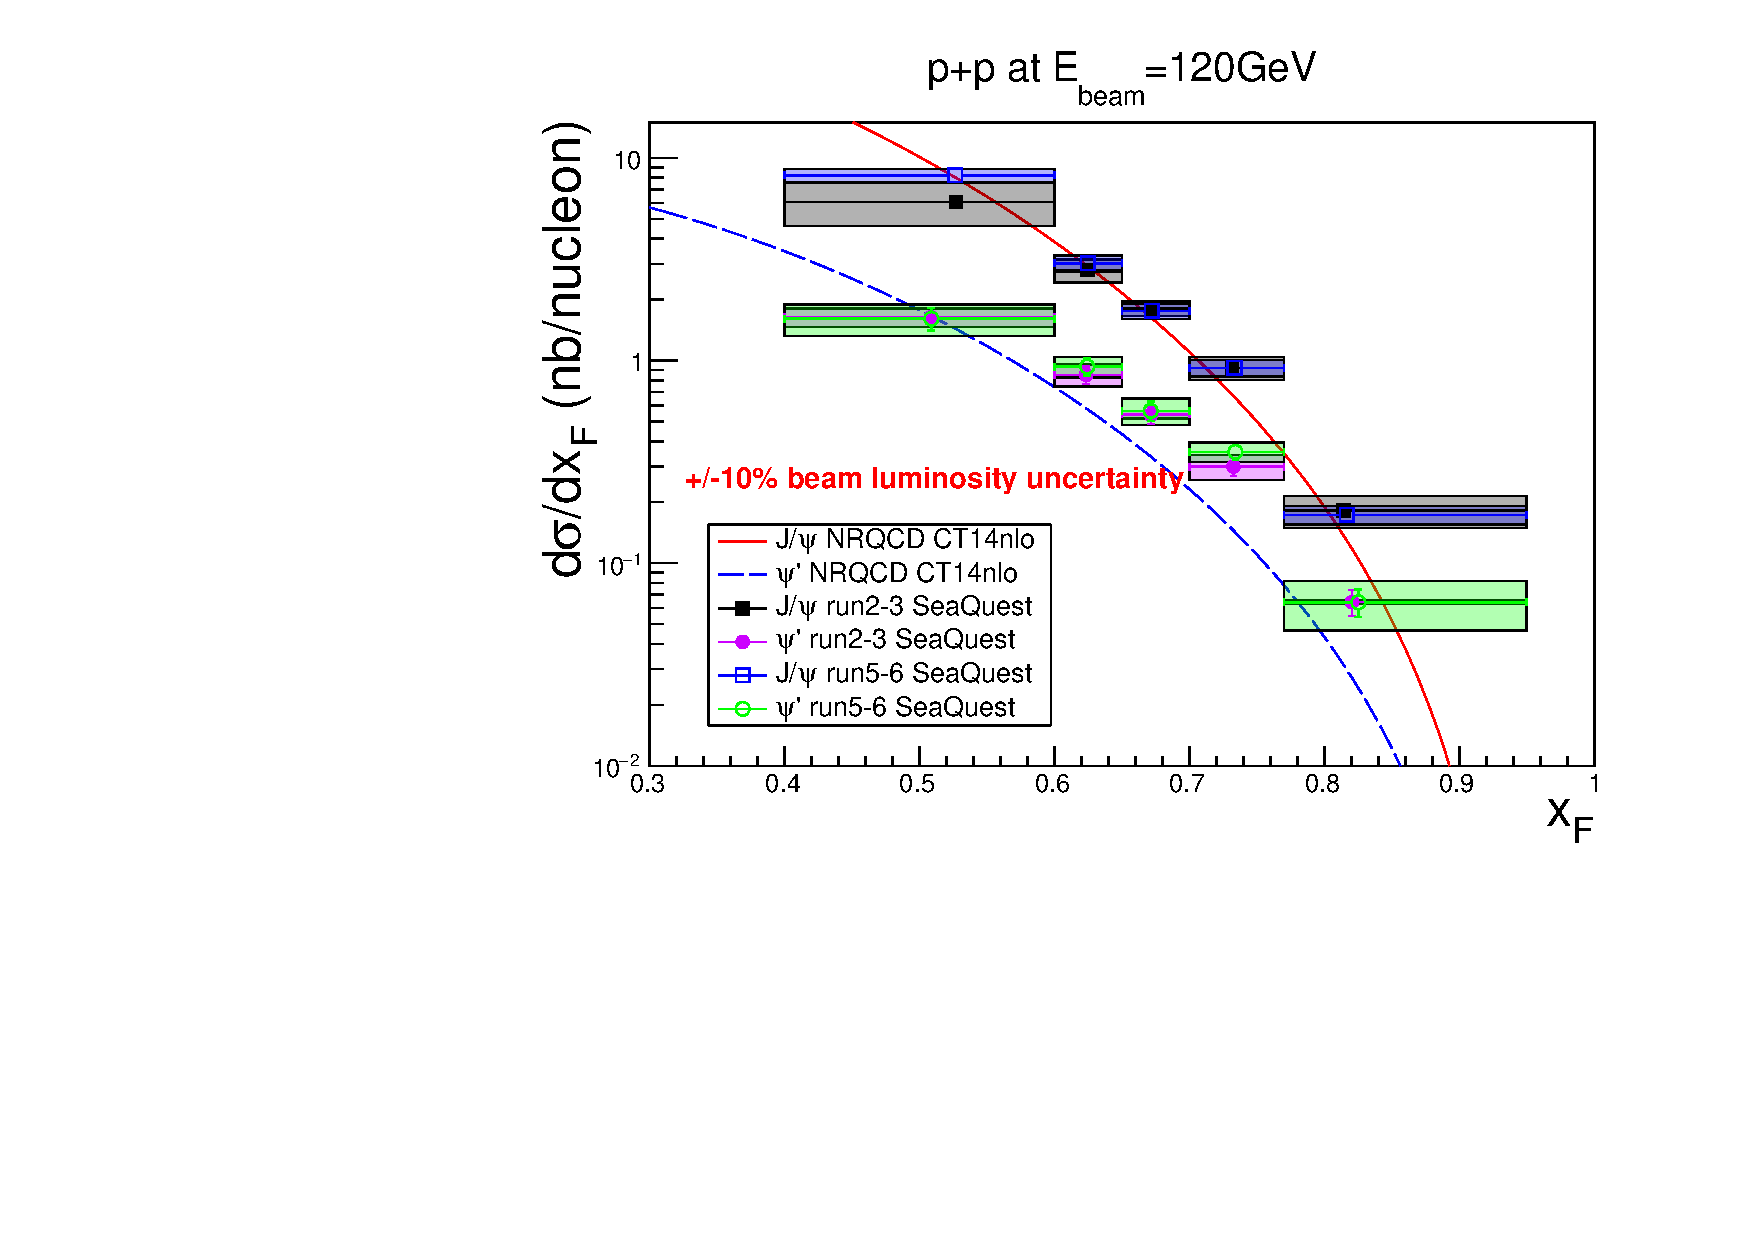
\includegraphics[width=\linewidth]{figures/crossSections/xF/combine_xF_LH2_5-6_5770_psip}
	\end{subfigure}
	\begin{subfigure}{0.45\linewidth}
		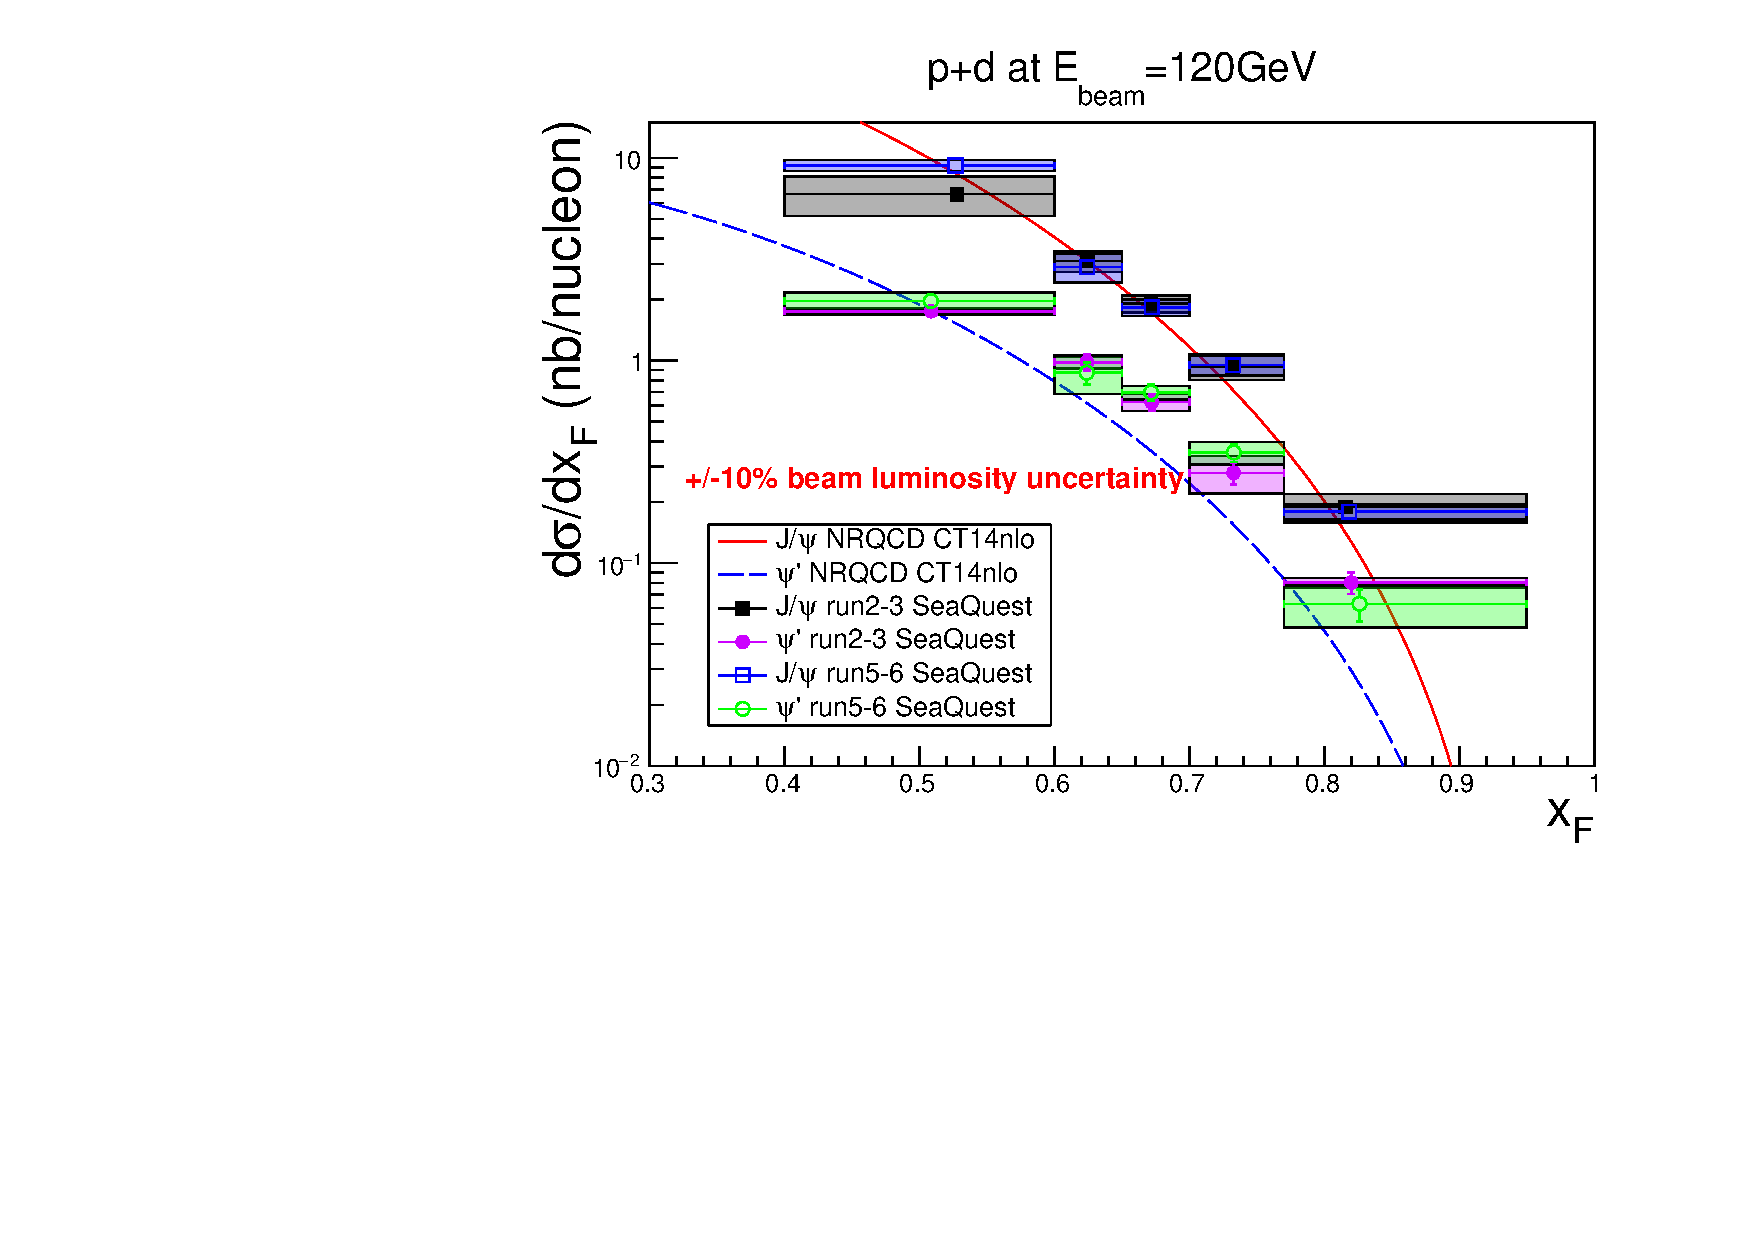
\includegraphics[width=\linewidth]{figures/crossSections/xF/combine_xF_LD2_5-6_5770_psip}
	\end{subfigure}
	\caption{The measured $d\sigma /d x_F$ for $J/\psi$ and $\psi'$. The curves correspond to NRQCD
		calculations using the LDMEs obtained from Ref.~\cite{hsieh2021} and the CT14 PDF.}
	\label{fig:xF_cross_sections}
\end{figure*}

\todo{Need detail of the NRQCD calculation.}
To compare the measured cross section for charmonium 
production with theoretical expectation, we have preform calculation
using the Next-to-Leading order (NLO) non-relativistic QCD (NRQCD)
framework \cite{bodwin1995}. The production of the $c\bar{c}$ pair proceeds
through a short-distance partonic interaction, calculated using perturbative QCD.
The probability of hadronization of a $c\bar{c}$ pair into some charmonium bound
state depends on its spin, color and angular momentum.
Being of a non-perturbative nature, the hadronization is described by the associated
long-distance matrix elements (LDMEs). The LDMEs used are taken from Ref.~\cite{hsieh2021}.

The magnitude and the shape of the extracted $J/\psi$ cross sections,
shown in \cref{fig:xF_cross_sections}, are in good agreement with the NRQCD calculation. 
However, the extracted $\psi'$ cross section is considerably wider than the expectation.
It is possible the LDMEs used in for the $\psi'$ cross section calculation is not fully optimized.
This new result on the $\psi'$ cross section can be used in further constrain the LDMEs. 

\todo{describe the $\sigma_{\psi'}/\sigma_{J/\psi}$ ratio\\
	the $\psi'$ distribution is expected to be wider than that of $J/\psi$ as the $q\bar{q}$ is more important
}
\begin{figure*}[h]
	\begin{subfigure}{0.45\linewidth}
		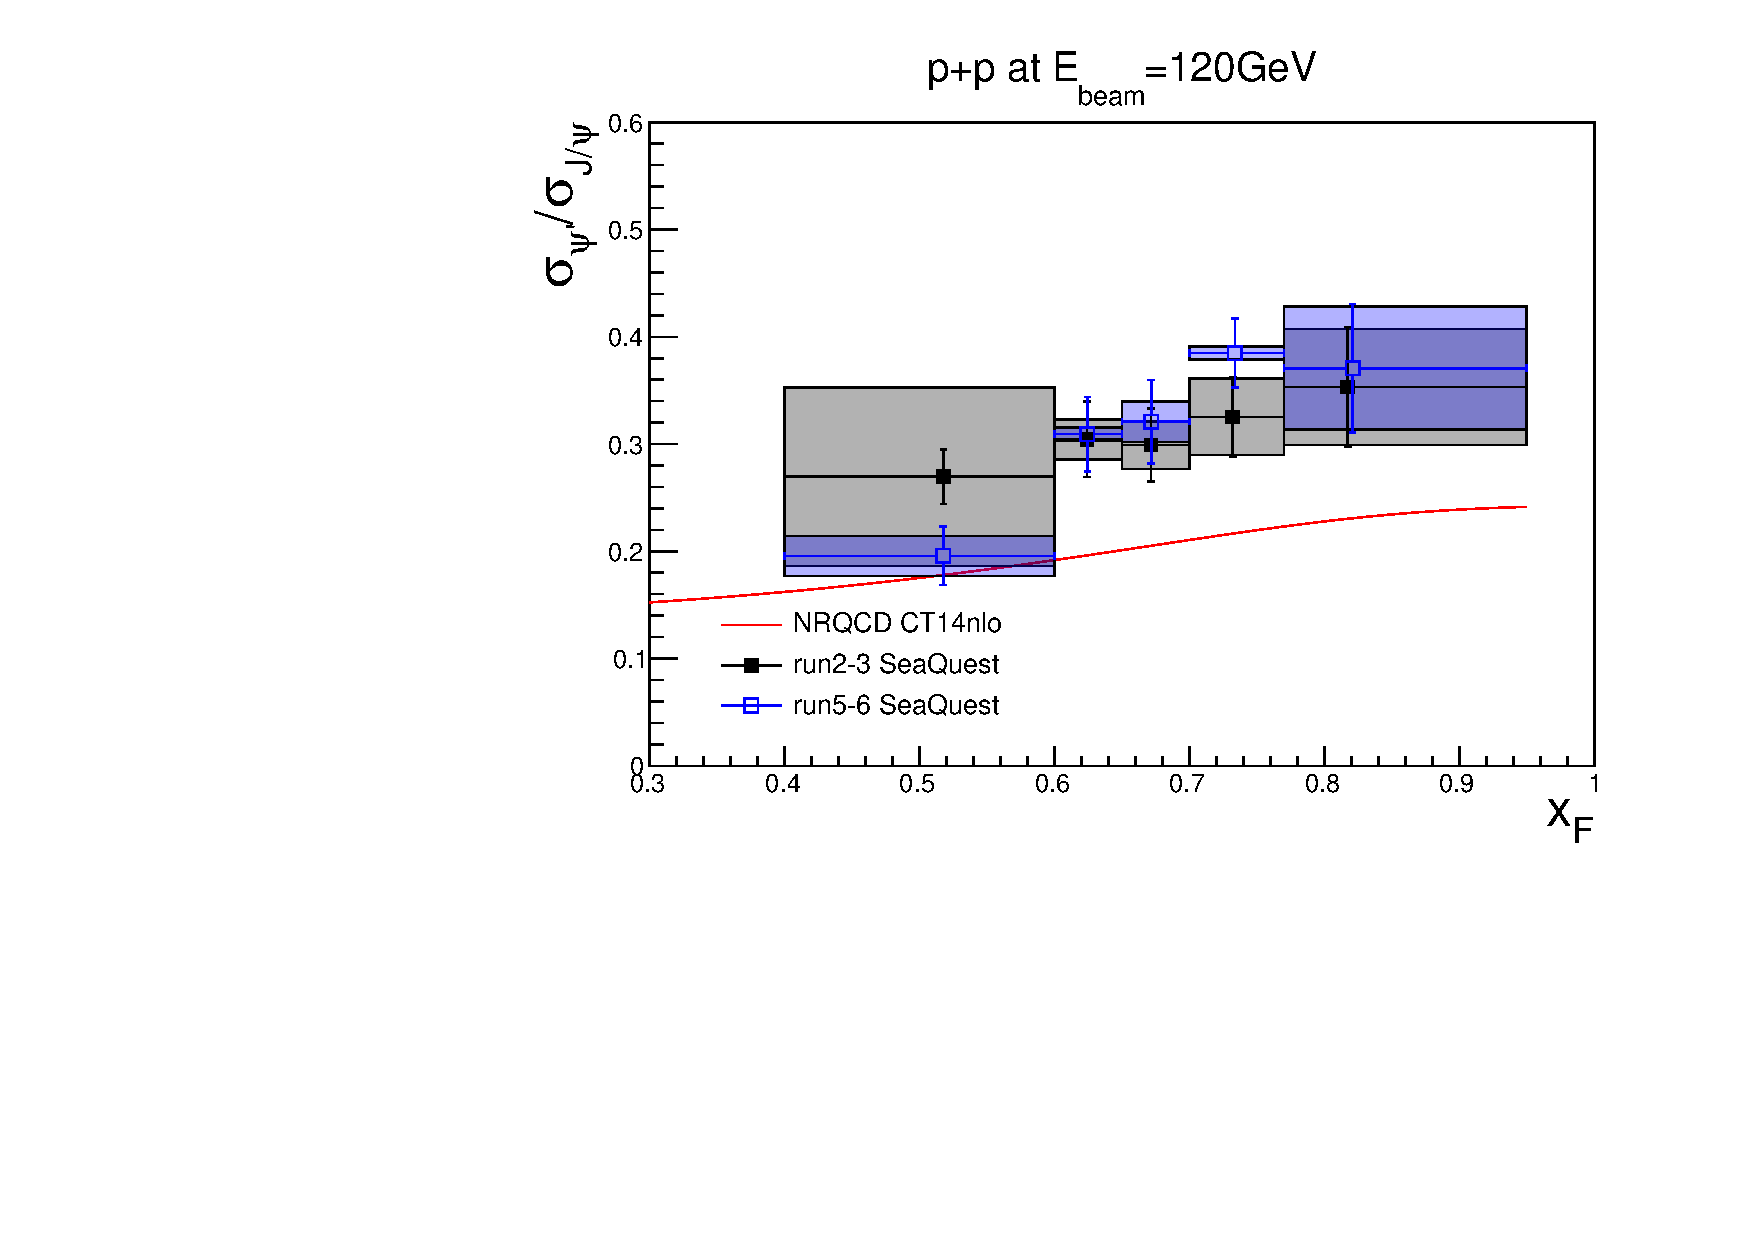
\includegraphics[width=\linewidth]{figures/crossSections/xF/ratio_xF_LH2_5-6_5770}
	\end{subfigure}
	\begin{subfigure}{0.45\linewidth}
		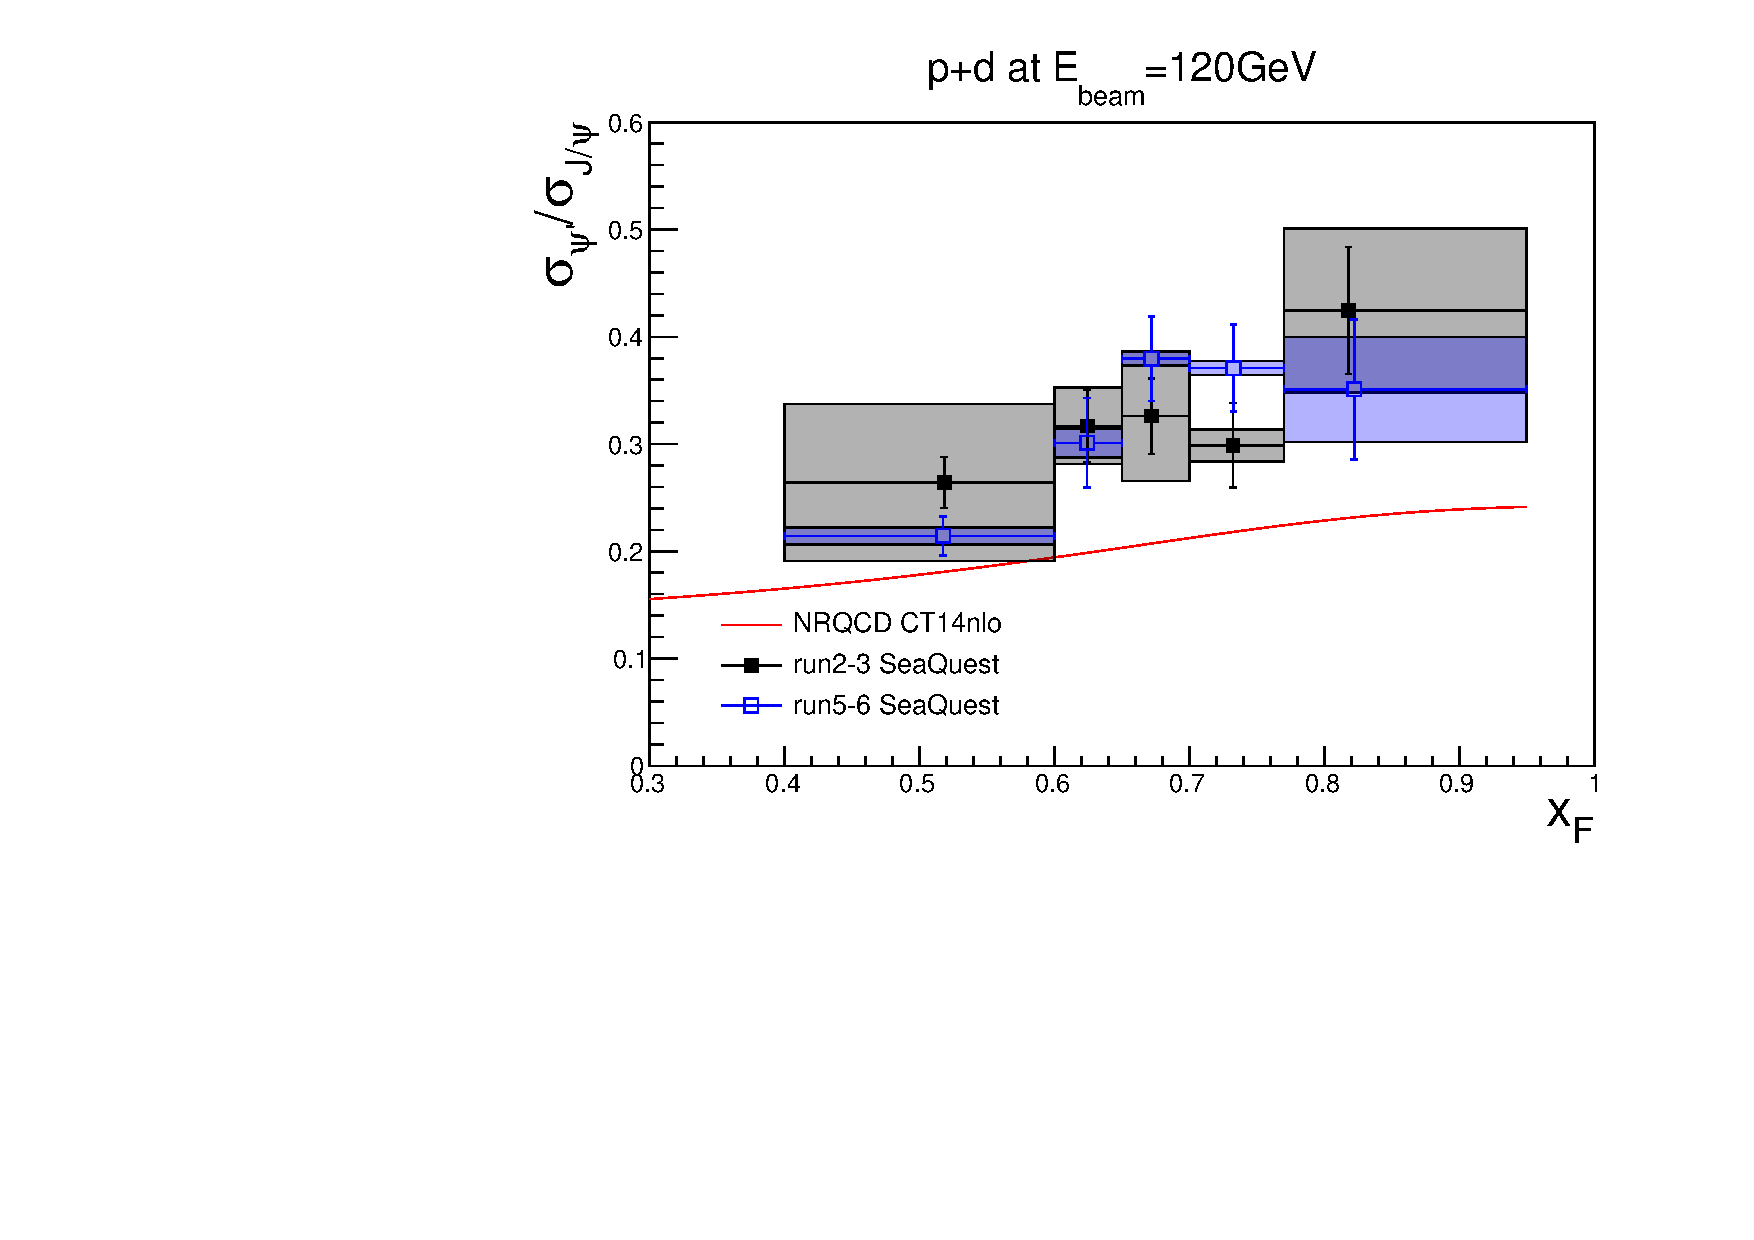
\includegraphics[width=\linewidth]{figures/crossSections/xF/ratio_xF_LD2_5-6_5770}
	\end{subfigure}
	\caption{The measured $\sigma_{\psi'}/\sigma_{J/\psi}$ ratio compared with NRQCD calculations}
	\label{fig:psip_jpsi_ratio_xF}
\end{figure*}
\Cref{fig:psip_jpsi_ratio_xF} shows to ratio of $\sigma_{\psi'}$ to $\sigma_{J/\psi}$.
The ratio shows a clear $x_F$ dependence, and the measured ratio increases as $x_F$ increases.
In the NRQCD framework, the difference in the $x_F$ distributions between $J/\psi$ and $\psi'$
is mostly originated from the relative weighting between the different production subprocess.
This result suggests the $q\bar{q}$ annihilation being more important in the $\psi'$ production
than the $J/\psi$.

\todo{described the $P_T$ distribution and the fit, need to add a table of $\expval{P_T}$}
\Cref{fig:pT_cross_sections} displays the differential charmonium production cross section $d\sigma/d P_T^2$
per nucleon versus the transverse momentum. The transverse momentum distributions are fitted to the
following function\cite{kaplan1978}
\begin{equation}
	f\left(P_T^2\right) \propto \frac{1}{\left(1+ P_T^2/p_1^2\right)^6},
	\label{eq:kaplan}
\end{equation}
The parameter $p_1$ controls the broadness of the $P_T$ distribution. And is
related to the average $P_T$ as follows
\begin{equation}
	\expval{P_T}    = \frac{35\pi p_1}{256}, \quad \mathrm{and}\quad
	\expval{P_T^2}  = \frac{p_1^2}{4}.
\end{equation}
\begin{figure*}[h]
	\missingfigure{$P_T$ distribution. Need to decide the format of the figure.}
	\caption{The measured $d\sigma/d P_T^2$ for $J/\psi$ and $\psi'$}
	\label{fig:pT_cross_sections}
\end{figure*}

\todo{The measured $\expval{P_T^2}$ vs $\sqrt{s}$ from different experiments}
\Cref{fig:pt_s} shows the extracted $\expval{P_T^2}$ for $p+p\rightarrow J/\psi$ as a function
of $\sqrt{s}$ from SeaQuest compared with different experiments
\cite{badier1983,clark1978,drapier1998,acharya2020}. The $\expval{P_T^2}$ follows an
increasing pattern versus $\sqrt{s}$ over a wide range of energies.
The data points are also fitted to the following form, taken from Ref.~\cite{acharya2020}.
\begin{equation}
	\expval{P_T^2}=a\ln{\left( \frac{\sqrt{s}}{b} \right)},
\end{equation}
with $a=1.221\pm0.038$ and $b=7.59\pm0.31$.
\begin{figure}
	\centering
	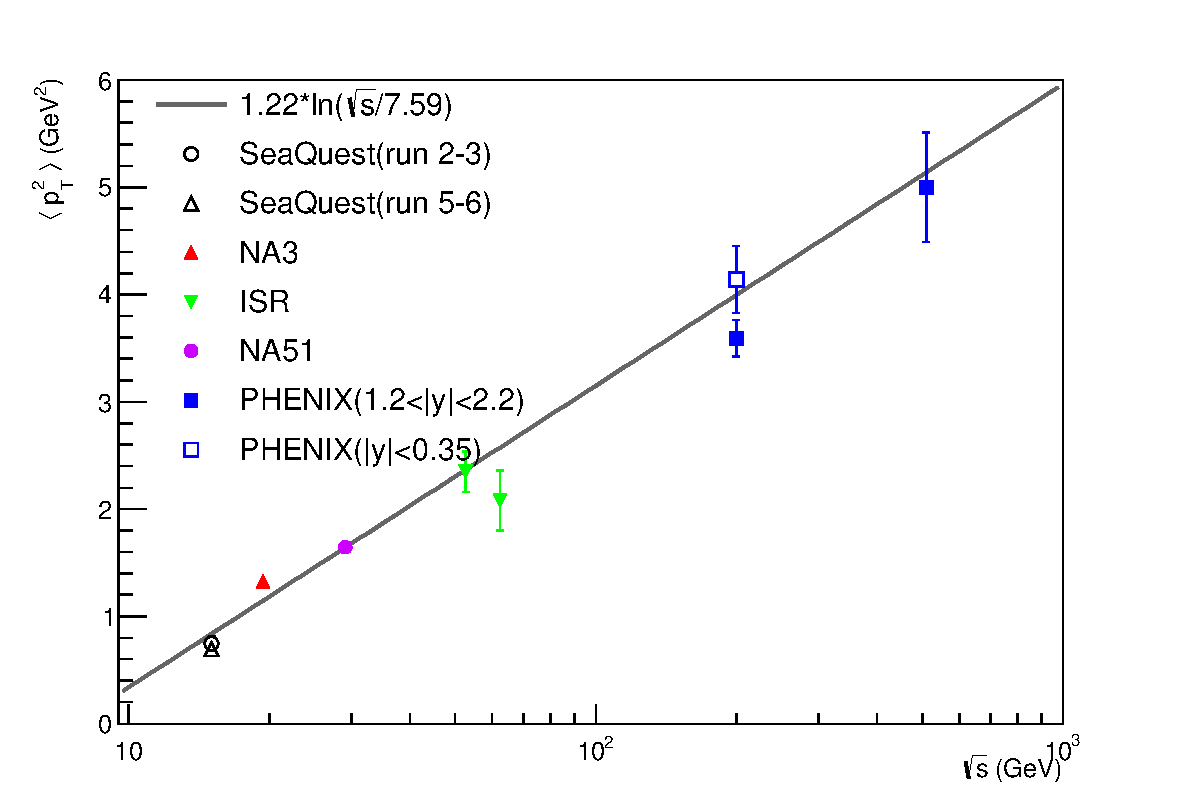
\includegraphics[width=\linewidth]{crossSections/pT/pT_s_release}
	\caption{The measured $\expval{P_T^2}$ from SeaQuest for $p+p\rightarrow J/\psi$ compared with other experiments \cite{clark1978,drapier1998,acharya2020}}
	\label{fig:pt_s}
\end{figure}

\section{$(p+d)/(p+p)$ Cross Section Ratio}
\label{sec:CSR}
\todo{comparison with NA51}
As a result of the identical target geometry
of the two liquid targets and the frequent interchange between the targets,
many of the systematic uncertainties encountered in evaluating $\sigma$
are correlated for the hydrogen and deuterium targets. Hence, most of these
systematic uncertainties cancel out in the ratio of $(p+d)/(p+p)$ cross
sections.

Shown in \cref{fig:pd/pp_csr} are the $(p+d)/(p+p)$ $J/\Psi$
and $\Psi^\prime$ cross section
ratios measured by the NA51 Collaboration~\cite{abreu1998} with 450 GeV proton
beam, covering a different region of $x_F$. Both the NA51 and the SeaQuest
results show the cross section ratios for $J/\Psi$ and $\Psi^\prime$
production are close to unity, in striking contrast to
the corresponding ratios for the Drell-Yan process~\cite{dove2023}, also
shown in \cref{fig:pd/pp_csr}. The difference between the Drell-Yan and the charmonium
cross section ratios clearly reflect the different underlying mechanisms in
these two processes.
\begin{figure}
	\missingfigure{$pd/pp$ cross section ratio vs $x_F$, compared with DY}
	\caption{The $pd/pp$ cross section ratio for Drell-Yan process, $J/\psi$ and $\psi'$}
	\label{fig:pd/pp_csr}
\end{figure}

\section{Conclusions}
\label{sec:Conclusions}

\nocite{*}
\bibliography{reference}
\end{document}
